\subsection{Implementation and Simulation}
The implementation of the economic MPC can be seen in \cref{app:Econ_MPC}.\\
In the simulation, the cost and the slack has been chosen to be the same for both pumps and outputs.
\begin{figure}[H]
    \centering
    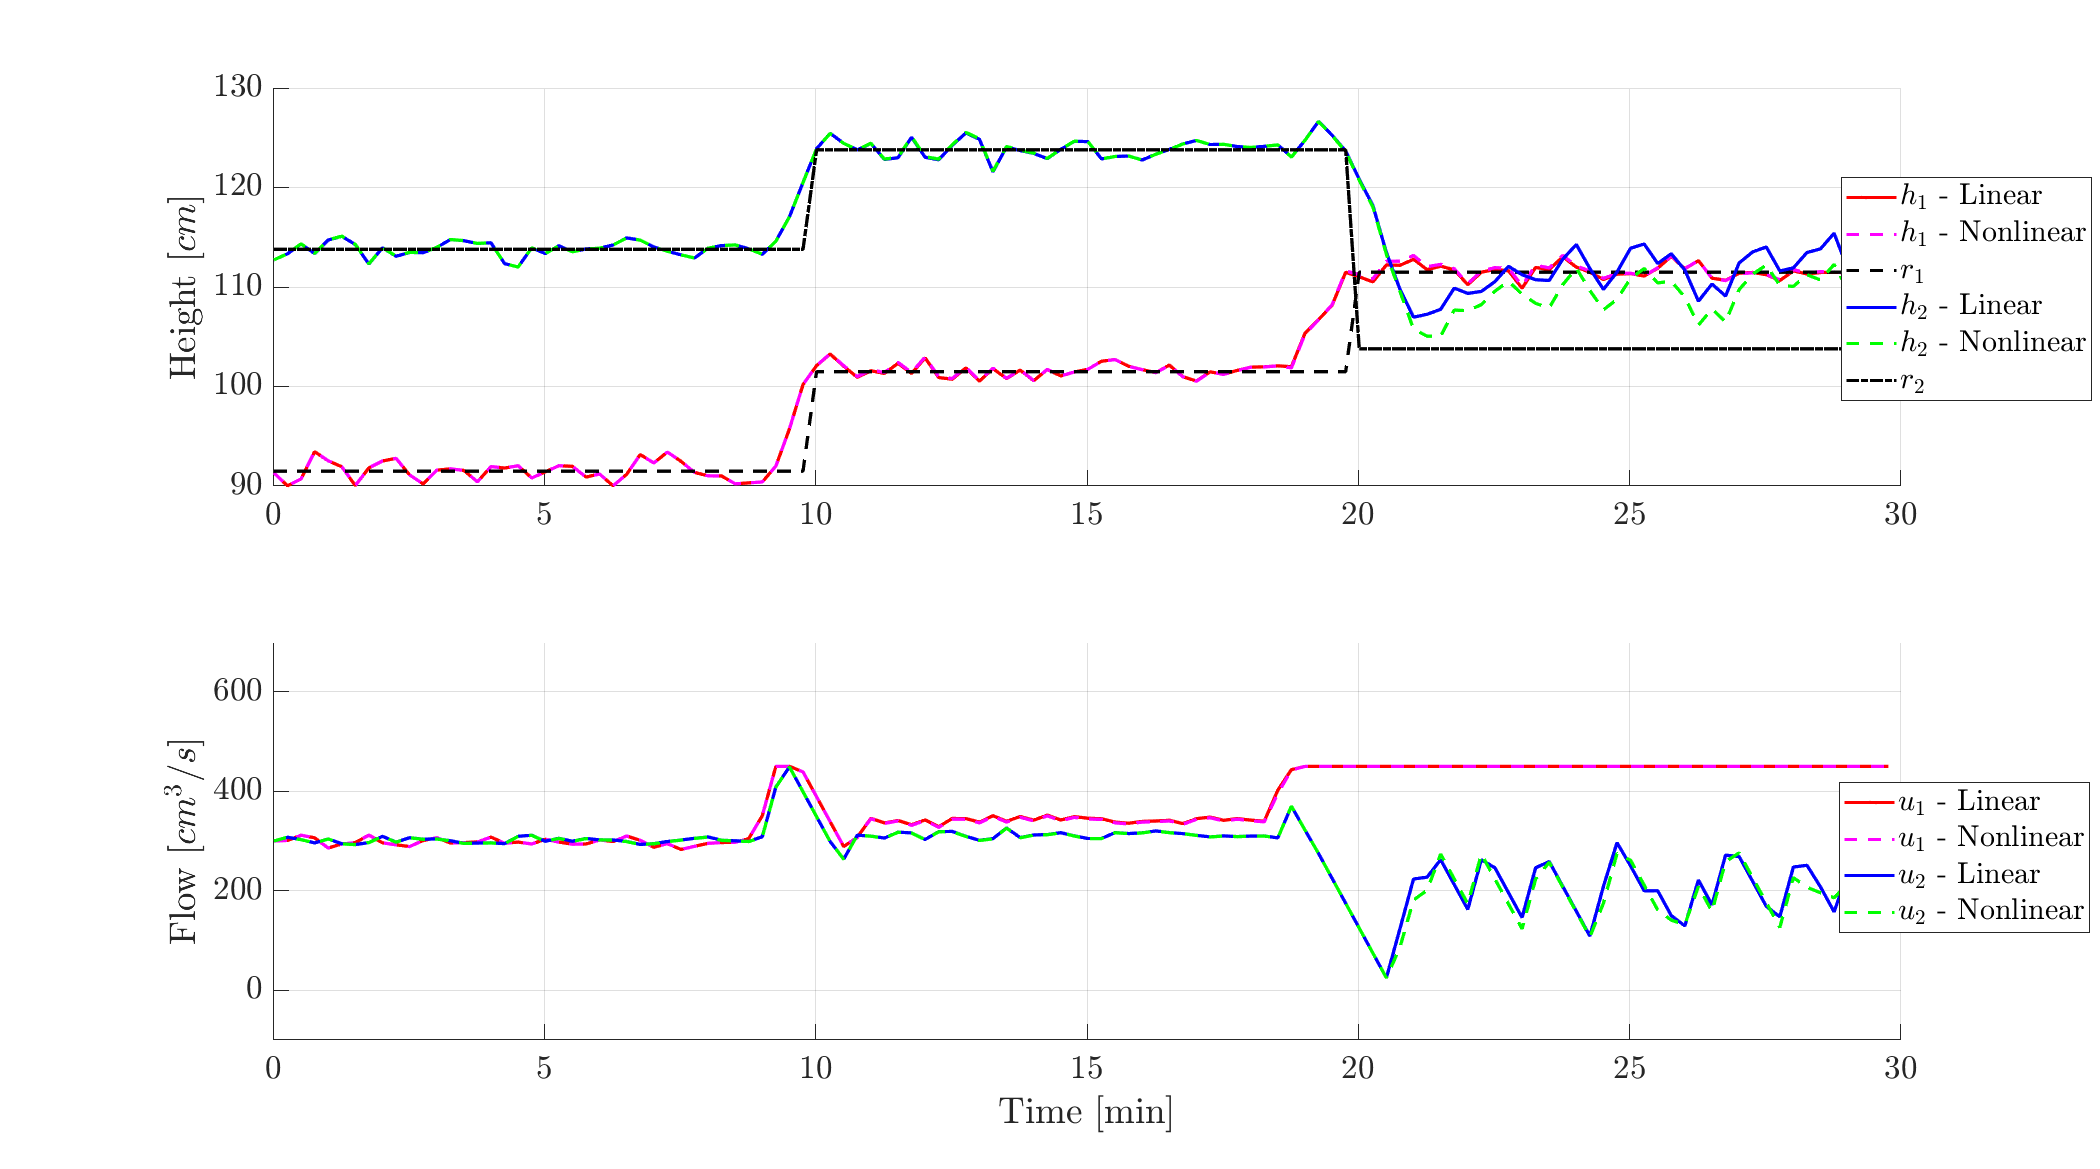
\includegraphics[width=1\textwidth]{Figures/Pr12.3_Econ_MPC.png}
    \caption{Economic MPC - Simulation}
    %\label{fig:Kalman_stoc_state_step}
\end{figure}
After 20 minutes, where the final step change in the reference occurs, the impact of the economic MPC can clearly be seen. The level in tank 2 is sufficiently close to the reference, and therefore the "on/off" effect on the pump occurs causing the input flow to vary.\\
The economic MPC differs significantly from the remaining MPC's designed in this project, since the economic MPC is a linear problem (where the remaining is a quadratic). If the cost of each pump is the same, the total flow is minimized, however if one of the pumps is evaluated to have a higher cost, the lowest cost pump could saturate. In these cases, the slack variable described previously would be different from 0.